\documentclass[a4paper,8pt,hyperref, twocolumn, aps, prl]{article}

\title{\bfseries \Large
%Surface second harmonic generated by submilliwatt pump
%Surface second-order nonlinear effects with ultralow power
%Ultralow-pumped surface second-harmonic generation in centrosymmetric medium
Surface second-harmonic generation enhanced by an ultrahigh-$Q$ microresonator
%of nonpolar media
}
\author{\normalsize  Xueyue Zhang$^{1,2}$, Qi-Tao Cao$^{1}$, Yu-xi Liu$^{2,3}$, Qihuang Gong$^{1,4}$, Yun-Feng Xiao$^{1,4,*}$ \\
  \\
\normalsize $^1$ State Key Laboratory for Mesoscopic Physics and School of Physics, Peking University \\
\normalsize Collaborative Innovation Center of Quantum Matter, Beijing 100871, People's Republic of China \\
\normalsize $^2$ Department of microelectronics and nanoelectronics, Tsinghua University, Beijing 100084, People’s Republic of China \\
\normalsize $^3$ Institute of Microelectronics, Tsinghua University, Beijing 100084, People’s Republic of China \\
\normalsize $^4$ Collaborative Innovation Center of Extreme Optics, Taiyuan 030006, Shanxi, People’s Republic of China \\
\normalsize $^*$ E-mail: yfxiao@pku.edu.cn
}
\date{\normalsize \today}

\usepackage[left=16mm,right=16mm, bottom = 16mm, top=20mm]{geometry}
\usepackage{upgreek}
\usepackage{hyperref}
\usepackage{booktabs}
\usepackage{tabularx}
\usepackage{xtab}
\usepackage{graphicx}
\usepackage{listings}
\usepackage{url}
\usepackage{amsmath}
%\usepackage{nature}



\lstset{
	flexiblecolumns,
	basicstyle = \sffamily,
	keywordstyle = \bfseries,
	commentstyle = \rmfamily\itshape,
	stringstyle = \ttfamily
}

\hypersetup{colorlinks=false}



%\pagestyle{myheadings}
%\markright{Name: Xueyue Zhang, GTID: 903181650}

\bibliographystyle{naturemag}

\begin{document}

\maketitle


\textbf{
Second-order nonlinear optical processes lie in the heart of many applications in both classical and quantum regimes, e.g. frequency conversion,  quantum squeezing and entanglement \cite{boyd2003nonlinear, pereira1988generation, kwiat1995new}.
Inversion symmetry, however, inhibits the second-order nonlinear dipole response in plenty of materials widely used in integrated photonics such as SiO$_2$, Si and Si$_3$N$_4$ \cite{boyd2003nonlinear, leuthold2010nonlinear, moss2013new}.
Symmetry breaking at surfaces/interfaces can produce second-order nonlinearity \cite{shen1989surface, heinz1991second, bloembergen1968optical, cazzanelli2016second}, but its signal typically requires high-power excitation and is hard to be distinguished from the contribution of bulk multipole nonlinearity \cite{heinz1991second, sun2015surface}.
Here, for the first time, we report second harmonic generation (SHG) originating deterministically from the surface nonlinearity of a silica microcavity.
The bulk multipole nonlinear effects are eliminated via pumping a mode with transverse electric polarization and confirming the even  field distribution of the SH mode in the polar direction, enabling the identification of surface nonlinear response.
The doubly resonant enhancement of ultrahigh-$Q$ cavity modes significantly lowers the pump power below one milliwatt, and boosts the SHG conversion efficiency to $0.049\%$ W$^{-1}$ which is around $14$ orders of magnitude higher compared with the non-resonance case \cite{tian2014recent}.
This work can trigger intense applications in ultra-sensitive surface analysis, extend the frequency conversion range of silica photonic devices and possibly push the surface nonlinear effects into the quantum regime.
}

The second-order nonlinearity in materials with inversion symmetry originates from both the asymmetric potential experienced by the surface/interface layer and the bulk multipole response beyond the electric-dipole approximation \cite{shen1989surface, heinz1991second}.
Different from breaking the bulk inversion symmetry, e.g., exerting external strain \cite{jacobsen2006strained, cazzanelli2012second} or electric field \cite{timurdogan2017electric}, the second harmonic (SH) and sum frequency generation (SFG) induced by the intrinsic surface nonlinearity have been developed as a non-invasive label-free probe, for example, to measure the arrangement,  adsorption or reaction of molecules on the surface \cite{sun2015surface, heinz1983determination, corn1994optical}.
%For , second harmonic and sum-frequency generation spectroscopy has been developed into a viable surface analytical tool
However, signals from surface nonlinear effects are extremely weak even under the high-intensity pump, typically only thousands of second-harmonic photons generated from a $50$-fs pulse with $500$ GW/cm$^{2}$ averaged intensity \cite{tian2014recent}.
Additionally, the bulk multipole second-order effects disturb the deterministic study of surface properties, which has long been highly challenging \cite{heinz1991second, tian2014recent}.

In the past decades, cavity-enhanced nonlinear optics with low pump power has witnessed dramatic development in whispering-gallery (WG) microresonators, with the demonstration of Raman laser \cite{spillane2002ultralow}, harmonic emission \cite{ilchenko2004nonlinear, carmon2007visible, furst2010naturally} and optical frequency combs \cite{del2007optical}.
The second-order nonlinear signal was also observed
in cavities made of centrosymmetric materials \cite{gouveia2013second, lettieri2002second, lettieri2005second, levy2011harmonic, asano2016visible, xue2017second}.
These studies, however, fail to clarify the surface second-order nonlinear effect and to operate under low pump power, both of which present obstacles in surface physics and further applications.
Here, we observe second harmonic, originating from surface-induced symmetry breaking and bulk multipole response (Fig. \ref{pic:Fig1}a), in a silica WG microsphere under the continuous wave pump below 1 mW.
The conversion efficiency of $0.049\%$ W$^{-1}$ results from the doubly resonant enhancement of ultrahigh-$Q$ modes (also known as the perfect phase match), which is achieved by thermal effect and optical Kerr effect.
We further confirm the surface-only SH signal, by analyzing the polarization dependence of the pump mode and the electric field distribution of the SH mode.

\begin{figure*}[!ht]
\centering
%\captionsetup{singlelinecheck=no, justification = RaggedRight}
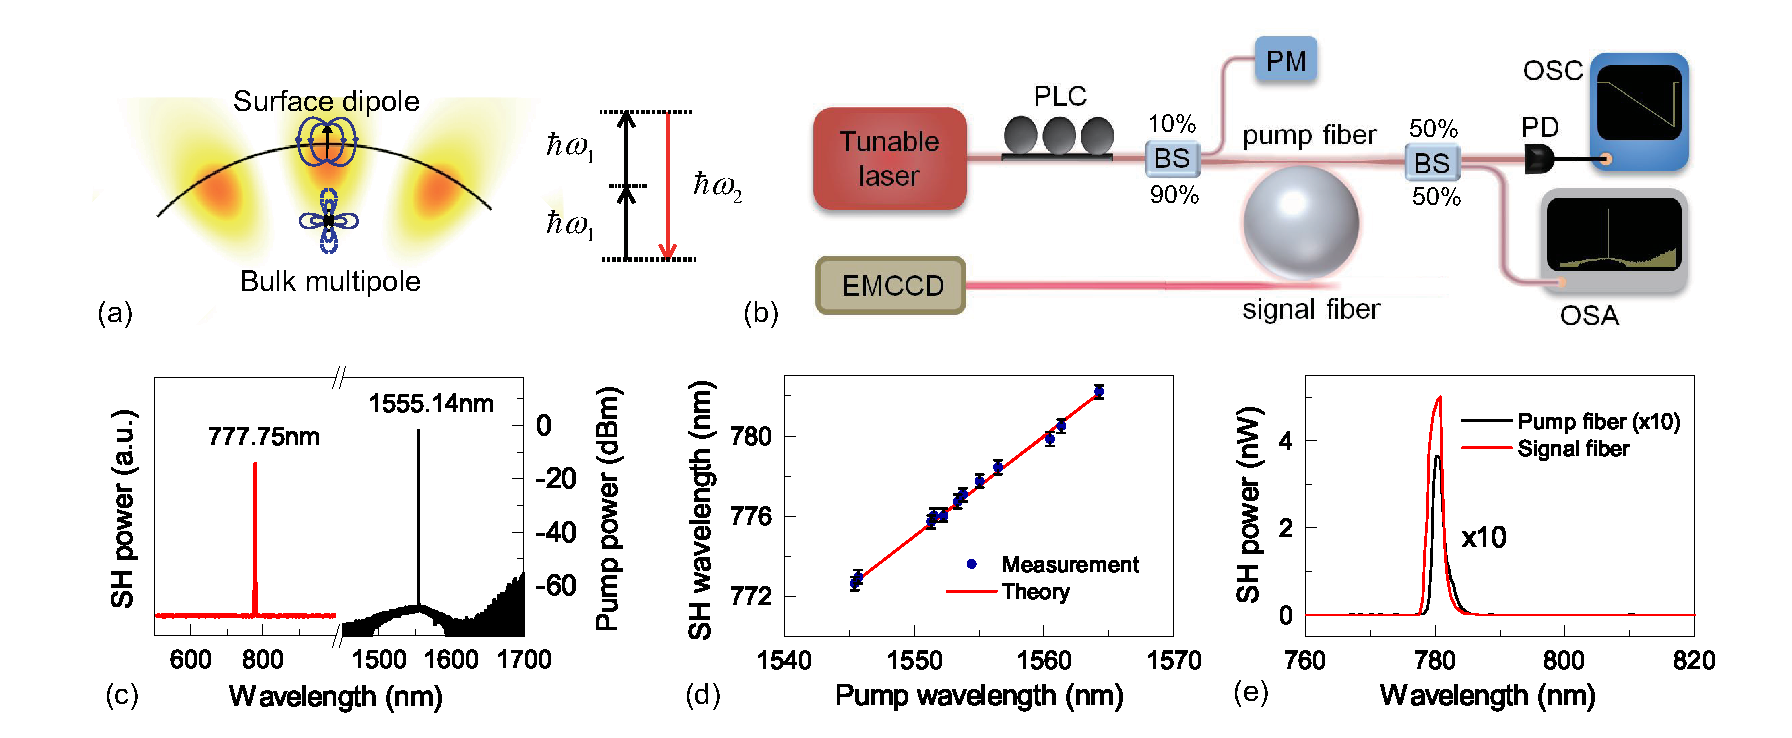
\includegraphics[width=18cm]{Fig1.eps}
\caption{\textbf{Experimental set-up and observation of cavity-enhanced SH signals. a, }SH is generated from the surface dipole response and the bulk multipole response in a WG microsphere. \textbf{b, }The pump light from a tunable laser around 1550 nm is coupled into a silica microsphere through a tapered fibre, and a second fibre is used to collect the SH signal. OSC: oscilloscope. OSA: optical spectrum analyzer. PLC: polarization controller. BS: beam splitter. EMCCD: electron-multiplying CCD. \textbf{c, }Measured SH spectrum (red) and the corresponding pump light (black). \textbf{d, } The blue dots stand for the measured SH wavelengths versus the corresponding pump wavelengths for different modes. The red line describes the rigorous $2\lambda_2 = \lambda_1$ dependence, where $\lambda_1$ ($\lambda_2$) denotes the wavelength of pump (SH) light.
\textbf{e, }Comparison of SH power collected by the signal fibre and the pump fibre (10 times magnified).}
\label{pic:Fig1}
\end{figure*}


In the experiment, a silica microsphere (diameter $\sim$ $62$ $\upmu$m)
is pumped through a tapered optical fibre (waist diameter $\sim$ $1$ $\upmu$m) at $1550$ nm band, as shown in Fig. \ref{pic:Fig1}b. To collect SH signal efficiently, a second fibre taper (waist diameter $\sim$ 0.5 $\upmu$m) designed for 780 nm band is incorporated into the system. The intrinsic quality factor for the pump cavity mode is $4.8\times10^7$.
Figure \ref{pic:Fig1}\textbf{c} shows a typical SH measured from the electron-multiplying CCD (EMCCD) spectrometer and the corresponding pump from the optical spectrum analyzer (OSA). The SH signal appears at $777.75$ nm when pumped at $1555.14$ nm, which deviates only $0.023$\% from the expected wavelength, falling into the resolution tolerance of OSA and EMCCD spectrometer.
Note that stimulated Raman scattering and parametric oscillation do not occur because their thresholds are far above the pump power in the experiment \cite{spillane2002ultralow, del2007optical}.
Third harmonic generation is also absent due to the phase mismatch in the nonlinear optical process \cite{carmon2007visible}.
Moreover, SH signals arise frequently when cavity modes are pumped from $1545$ nm to $1565$ nm, as shown in Fig. \ref{pic:Fig1}d.
Among the occurrence of SH, a maximum signal power of $5$ nW is observed via the signal fibre. 
To compare the collecting efficiencies of the two fibres, we optimize the fibre-cavity coupling so that the SH signal from the pump fibre is also observable, but its maximum signal power is still over one order of magnitude weaker than that from the signal fibre. From either fibres, SH signal is absent when the pump is off-resonance with cavity modes, which helps to eliminate the possibility of spurious signals such as the second-order diffraction of the EMCCD grating.


The doubly resonant enhancement plays a pivotal role in efficient SHG, which is achieved by perfect phase-matching including momentum conservation and energy conservation \cite{boyd2003nonlinear}.
The former can be fulfilled by a pair of modes with proper angular momentum relation $m_2=2m_1$, where $m_1$ ($m_2$) is the azimuthal number of the pump (SH) cavity mode.
The material and geometric dispersion presents a challenge on energy conservation, obstructing the double resonance $\omega_2=2\omega_1$ and consequently, efficient SHG.
More accurately, the SH power can be derived from coupled mode equations (see Supplementary Information)
\begin{equation}
P_2 = \frac{4|g|^2\kappa_{2e}Q_2^2/\omega_2^2}{4Q_2^2(2\omega_p/\omega_2-1)^2+1}\frac{16\kappa_{1e}^2Q_1^4/\omega_1^4}{[4Q_1^2(\omega_p/\omega_1-1)^2+1]^2}P_1^2,
\label{eq:P2P1}
\end{equation}
where the subscripts $j=1, 2$ represent the pump cavity mode and SH mode respectively with $\omega_j$ being the resonant frequency and $Q_j$ the loaded quality factor, $\omega_p$ and $P_1$ denotes the pump frequency and power respectively, $g$ is the second-order nonlinear coupling strength between the two modes, and $\kappa_{je}$ represents the external coupling rate. The pump power depletion is ignored due to the weak second-order nonlinear effect in silica.
Equation (\ref{eq:P2P1}) shows that ultrahigh $Q$ is indispensable in boosting the SH power, while the corresponding ultra-narrow linewidth also presents a challenge to achieve the double resonance.  %due to the aggravated influence of frequency mismatch.
In order to compensate the dispersion, the delicate geometric control and the integration of fine nanostructures are proposed in the cavities \cite{levy2011harmonic, kozyreff2008whispering, xu2008second, dominguez2011whispering}, but challenging for an ultrahigh-$Q$ (ultra-narrow-linewidth) microresonator.
To tune the cavity dispersion precisely and dynamically, we leverage the cavity-enhanced thermal and optical Kerr effects to manipulate the frequencies of both pump and SH cavity modes.


\begin{figure*}[!ht]
\centering
%\captionsetup{singlelinecheck=no, justification = RaggedRight}
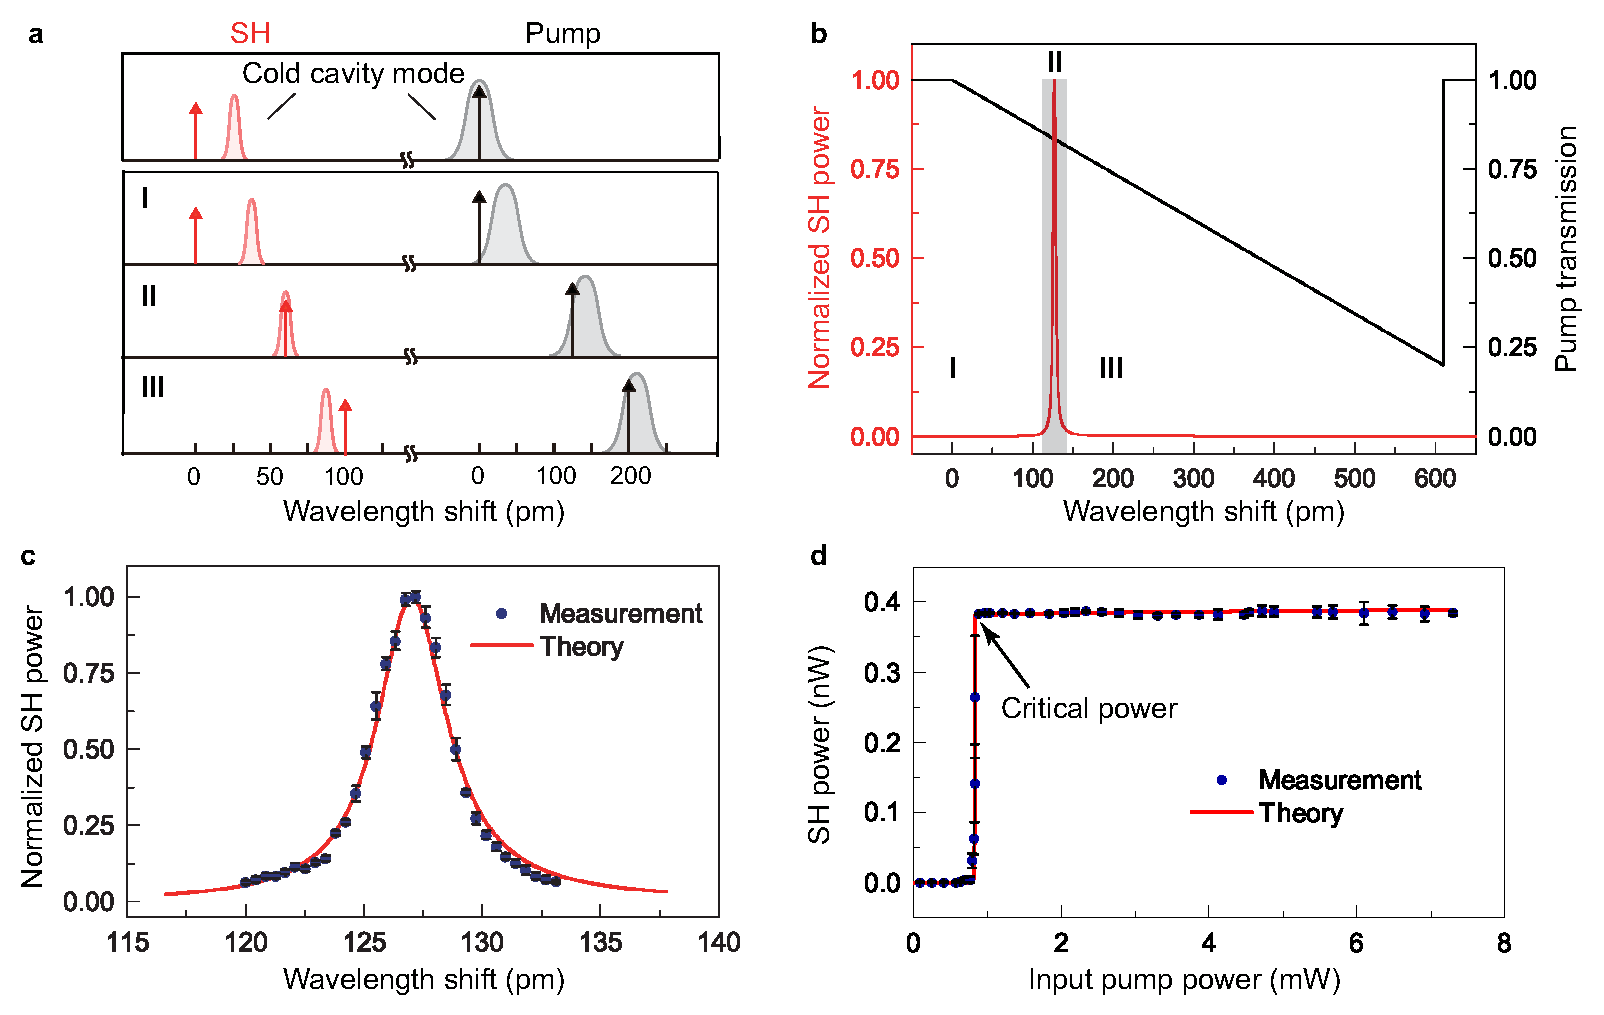
\includegraphics[width=17cm]{try_ed3.eps}
\caption{\textbf{Perfect phase matching assisted by thermal and Kerr effects. a, }Schematic of the phase-matching process.
%Detuning here is the wavelength relative to the cold-cavity wavelength of the pump mode (to half of this wavelength for SH detuning).
The black (red) arrows represent the pump light (its SH). The grey (red) Lorentzian shape stands for the pump (SH) cavity mode. States
\textbf{I}  - \textbf{III}  show three cases with increasing pump wavelength but the same input power. 
\textbf{b, }Theoretical SH power (red curve) and pump transmission (black curve) at different pump wavelength shift relative to the cold-cavity mode. \textbf{I} - \textbf{III} correspond to the three states in \textbf{a}. % The grey area is enlarged in \textbf{c}. 
\textbf{c, }SH power versus pump wavelength shift with the input power of 4.46 mW. The wavelength range is the same as that of the grey area in \textbf{b}.
\textbf{d, }The dependence of maximum SH power on the input power for the same pump mode.}
\label{pic:Fig2}
\end{figure*}


The mechanism of thermal and Kerr assisted phase matching process is illustrated in Fig. \ref{pic:Fig2}a.
When the pump is weak and on resonance with the cold cavity mode ($\omega_{10}$), the SH mode ($\omega_{20}$) is unlikely to be on resonance with the SH signal because of the dispersion, as shown in the top panel of Fig. \ref{pic:Fig2}a.
With a high enough input power, both the pump and SH modes experience red shifts due to the thermal and Kerr effects of the pump light, which can be described by $\omega_1-\omega_{10} = -B_{11}|\alpha_1|^2$ and $\omega_2-\omega_{20} = -B_{12}|\alpha_1|^2$, respectively. Here $|\alpha_1|^2$ is the intracavity energy of the pump mode, $B_{11}$ and $B_{12}$ denote the coefficients.
The thermal and Kerr effects of the SH are ignored in the analysis.
%The SH mode also exhibits a red shift from the cold cavity frequency, which can be described by $\omega_2-\omega_{20} = -B_{12}|\alpha_1|^2$ with the coefficient $B_{12}$.
In this case, the wavelength of pump light should increase to catch the pump mode, forming the non-Lorentzian shape in pump transmission (black curve in Fig. 2b).
%resulting in the non-Lorentzian, triangular transmission shape \cite{carmon2004dynamical}, as shown in the black curve in Fig. \ref{pic:Fig2}b.
%The SH mode also exhibits a red shift from the cold cavity frequency, which can be described by $\omega_2-\omega_{20} = -B_{12}|\alpha_1|^2$ with the coefficient $B_{12}$.
With increasing pump wavelength, the SH signal moves faster than the SH mode considering the temperature distribution in the cavity (see Supplementary Information).
In the process of tuning pump light towards the pump mode (states \textbf{I} - \textbf{III} in Figs. \ref{pic:Fig2}a and b), the SH signal can catch the SH mode ($\omega_2$) at a certain pump wavelength.
The phase-matching condition is fulfilled in this case, and thus the SH power reaches a peak value (state \textbf{II}).
By further increasing the pump wavelength, the SH signal passes the SH mode, and its power diminishes rapidly (state \textbf{III} in Figs. \ref{pic:Fig2}a and b).
In the experiment we tune the pump frequency in the range of the grey area in Fig. \ref{pic:Fig2}b with a given input power, and consequently obtain the SH power as the blue dots shown in Fig. \ref{pic:Fig2}c, which agree with the theoretical prediction.
%Note that under a certain input power both the pump and SH can be completely resonant with cavity modes respectively , where SH power is just able to arrives at the peak value in Fig. \ref{pic:Fig2}b.


Furthermore, the dependence of SH power on pump power is studied, as presented in Fig. \ref{pic:Fig2}d.
Experimentally, under each input power, we search for the strongest SH output by tuning the pump wavelength within the pump mode.
Among different input power, a critical power manifests itself, at which the pump and the SH are exactly on resonance with the respective cavity modes.
%In this case, the SH power is able to arrives at the peak value in Fig. \ref{pic:Fig2}c, which represents the most efficient SHG with the pump power of $879$ $\upmu$W and the conversion efficiency of $0.049\%$ W$^{-1}$.
In this case, the efficient SHG with the pump power of $879$ $\upmu$W exhibits an unprecedented conversion efficiency of $0.049\%$ W$^{-1}$, which is enhanced by over $14$ orders of magnitude compared with the non-resonance case reported in \cite{tian2014recent}.
Below the critical input power, the SH is off resonance within the full tuning range, resulting in the extremely weak SH power.
Above the critical power, the increasing input power at a given frequency pushes the pump mode farther to the red side (the pump is not completely on resonance) and consequently increases the detuning between the pump light and the cavity mode.
The reduced enhancement of the pump light counteracts with the increasing input power, leading to the almost steady intracavity energy.
The on-resonance wavelength of the SH mode also remains stable so that the intracavity energy and consequently the SH power at this wavelength are almost the same as well (see Supplementary Information).
It is also possible to obtain the explicit $P_2 \propto P_1^2$ dependence by introducing a new degree of freedom, such as a control light or a heater, to manipulate the SH mode frequency.

\begin{figure*}[!ht]
\centering
%\captionsetup{singlelinecheck=no, justification = RaggedRight}
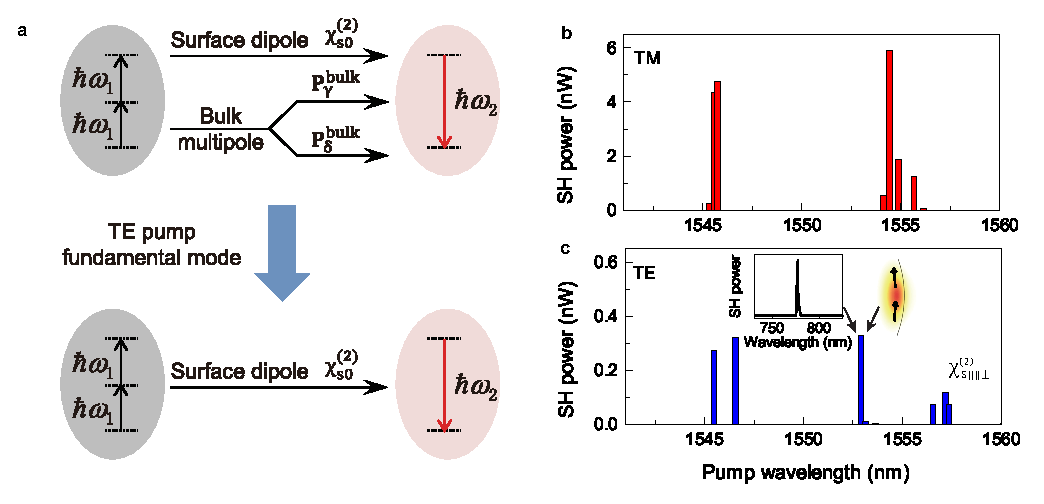
\includegraphics[width=16cm]{Fig3new.eps}
\caption{\textbf{Identification of surface nonlinearity from the bulk multipole response. a, }Origin of second-order nonlinearity and the approach to obtain surface-only nonlinear coupling. \textbf{b, c,} Second harmonic power measured with TM (\textbf{b}) and TE (\textbf{c}) pump polarization respectively, in the pump wavelength range from 1541 nm to 1560 nm. Inset in \textbf{c}: Measured second harmonic spectrum (left), and the polar field distribution of the target SH mode (right).}
\label{pic:Fig3}
\end{figure*}

In order to distinguish the contributions of surface and bulk nonlinearity, we investigate the polarization dependence in SHG.
In equation (\ref{eq:P2P1}), The surface dipole contribution to the nonlinear coupling strength can be written as (see Supplementary Information)
\begin{equation}
g_{s0} = 2\frac{\omega_1^2}{\omega_2n^2}\frac{\int_{\mathrm{surface} } \mathbf{E}_{02}^* \cdot \upchi^{(2)}_{s0}:\mathbf{E}_{01}\mathbf{E}_{01} \mathrm{d}	\mathbf{S}}{\int |\mathbf{E}_{02}|^2 \mathrm{d}	\mathbf{V}}
\end{equation}
where $\upchi^{(2)}_{s0}$ represents the surface nonlinear susceptibility, $\mathbf{E}_{0j}(\mathbf{x})$ denotes the  normalized electric field, and $n$ is the refractive index of the cavity material.
The bulk multipole nonlinear polarization in silica, on the other hand, can be expressed as $\mathbf{P}^{\mathrm{bulk}} = \mathbf{P}^{\mathrm{bulk}}_\gamma + \mathbf{P}^{\mathrm{bulk}}_\delta = \gamma\nabla(\mathbf{E}\cdot\mathbf{E})+\delta(\mathbf{E}\cdot\nabla)\mathbf{E}$ \cite{bloembergen1968optical}, where $\gamma$ and $\delta$ are the nonlinear coefficients. The first term $\mathbf{P}^{\mathrm{bulk}}_\gamma$ represents a longitudinal wave which can excite SH only at the surface. Therefore $\mathbf{P}^{\mathrm{bulk}}_\gamma$ together with the surface dipole contribute to an effective surface susceptibility \cite{heinz1991second} $\upchi^{(2)}_s = \upchi^{(2)}_{s0}+\upchi^{(2)}_{s,\gamma}$, corresponding to an effective coupling strength of $g_s$. The coupling strength induced by the second term $\mathbf{P}^{\mathrm{bulk}}_\delta$ can be written as
\begin{equation}
g_b =  2\frac{\omega_1^2}{\omega_2n^2}\frac{\delta \int \mathbf{E}_{02}^* \cdot (\mathbf{E}_{01}\cdot\nabla)\mathbf{E}_{01} \mathrm{d}	\mathbf{V}}{\int |\mathbf{E}_{02}|^2 \mathrm{d} \mathbf{V}}
\label{eq:gb}
\end{equation}
Thus the total second-order nonlinear coupling strength $g = g_s+g_b$, as shown in Fig. \ref{pic:Fig3}a.

The effective surface susceptibility tensor $\upchi^{(2)}_s$ consists of three non-zero components $\upchi_{\perp \perp \perp}$, $\upchi_{\parallel \parallel \perp}$ and $\upchi_{\perp \parallel \parallel}$ \cite{heinz1991second}, where $\perp$ ($\parallel$) denotes the electric field direction perpendicular (parallel) to the surface.
$\upchi_{\perp \parallel \parallel}$ can be ignored in studying SHG due to the non-degeneracy of transverse magnetic (TM) and  transverse electric (TE) pump modes.
$\upchi_{\perp \perp \perp}$ ($\upchi_{\parallel \parallel \perp}$) plays a major role when TM (TE) mode is pumped, which only generates the TM polarized second harmonic in both cases.
TM modes are preferable in surface induced SHG because $\upchi_{\perp \perp \perp}$ is stronger than $\upchi_{\parallel \parallel \perp}$ \cite{rodriguez2008calibration}.
Considering the bulk nonlinear response induced by $\mathbf{P}^{\mathrm{bulk}}_\delta$, the coupling strength $g_b$ relies on the specific field distribution in the cavity and the generated SH exhibits the same polarization as the pump mode.
Note that for TE polarization, the  electric field is along the polar direction, so that the polar symmetry of modes prohibits the excitation SH modes with an even polar distribution from $\mathbf{P}^{\mathrm{bulk}}_\delta$ (see Supplementary Information).
While the TM pump modes, with the electric field along the radial direction, can excite second harmonic without the above restriction.
Because of a stronger confinement in the radial direction than the polar direction and thus a larger gradient for most of the modes, TM modes tend to link with a larger $g_b$ than TE modes.
Consequently, from both the surface and the bulk second-order nonlinearity, the SH signals from TM pump modes are one or two magnitudes stronger than those from TE pump modes statistically (see Supplementary Information).
In the experiment, TM or TE modes from $1541$ nm to $1560$ nm are pumped separately by adjusting the polarization of the pump light.
The TM pump modes exhibit a much stronger SH power than TE mode by around one order of magnitude, as shown in Figs. \ref{pic:Fig3}b and c, as expected by the theoretical analysis.


The polarization dependence can be utilized to identify the surface nonlinearity from the bulk nonlinear response of both $\mathbf{P}^{\mathrm{bulk}}_\gamma$ and $\mathbf{P}^{\mathrm{bulk}}_\delta$.
The former can be removed by selectively pumping a TE polarized mode since $\upchi^{(2)}_{s,\gamma}$ is absent in the susceptibility $\upchi_{\parallel \parallel \perp}$ \cite{heinz1991second}.
The latter can be discerned from the surface nonlinear response with a TE pump mode, where an SH mode with even polar field distribution or TM polarization is forbidden to couple with the pump mode mediated by the $\mathbf{P}^{\mathrm{bulk}}_\delta$ as analyzed above.
%While the surface nonlinearity bridges the 
In the experiment, a surface-only SH (left inset in Fig. \ref{pic:Fig3}c) is obtained deterministically by employing a TE pump mode at 1553.07 nm and selecting the even polar field distribution of the SH mode. %, as shown in the right inset in Fig. \ref{pic:Fig3}c.
Here the SH mode distribution is confirmed experimentally by measuring the SH intensity while scanning the relative angular position of the signal fibre and the cavity, as illustrated in the right inset of Fig. \ref{pic:Fig3}c.
Alternatively, $\mathbf{P}^{\mathrm{bulk}}_\delta$ can also be eliminated by measuring the polarization of the SH signal (see Supplementary Information).

\begin{figure}[!ht]
\centering
%\captionsetup{singlelinecheck=no, justification = RaggedRight}
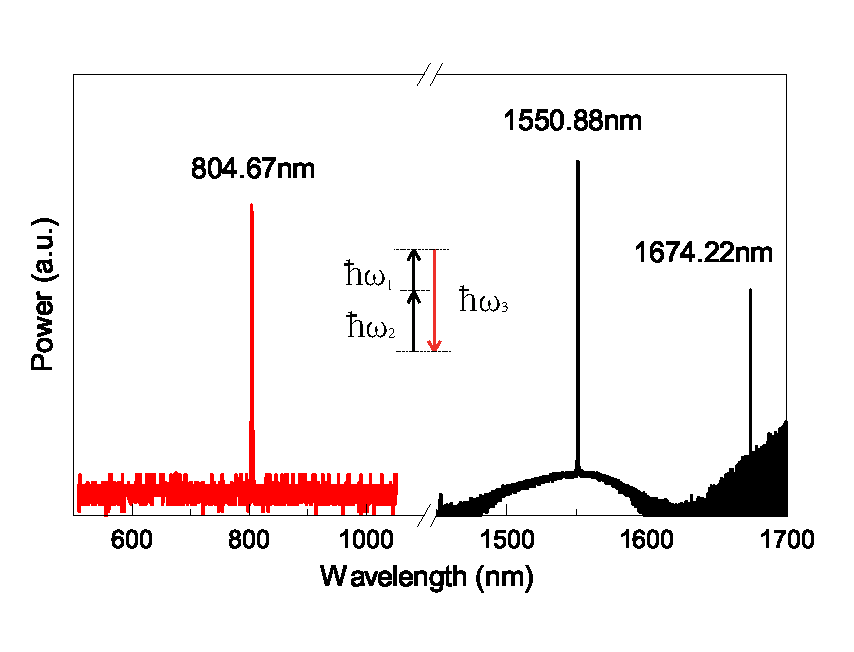
\includegraphics[width=8cm]{Fig4.eps}
\caption{\textbf{Measured spectra of second-order sum frequency generation. }The pump light ($\omega_1$) and Raman light ($\omega_R$) are summed to generate the SF signal ($\omega_2$) with an input power of $7.33$ mW.}
\label{pic:Fig4}
\end{figure}

With the second-order nonlinearity demonstrated above, sum frequency generation also arises, assisted by a Raman signal.
Shown in Fig. \ref{pic:Fig4} is a sum-frequency signal ($804.67$ nm), with the corresponding pump ($1550.88$ nm) and the stimulated Raman scattering ($1674.22$ nm).
The deviation of the sum-frequency wavelength from the expected value ($804.63$ nm) is much smaller than the resolution of the spectrometers.

For the first time, to the best of our knowledge, the second harmonic from the breaking of inversion symmetry at surface is deterministically observed in a silica microresonator without the influence of bulk multipoles.
This work opens up a new direction to focus on the surface nonlinearity with double resonance enhancement, where the detectable SH signal under submilliwatt pump power enables the study of surface properties and the detection of molecules with unprecedented sensitivity.
Moreover, the phase-matching method we used does not rely on the specific geometry and material of the cavity, making it a universal tool to develop surface nonlinear optics in various microcavity systems such as on-chip microtoroids, microdisks and microrings with different centrosymmetric materials like Si and Si$_3$N$_4$.
This work also shows great potential in studying CMOS-compatible quantum optics mediated by the second-order nonlinearity.

\bigskip
\noindent \textbf{\large Methods}

\noindent \textbf{Cavity fabrication and dual-fibre coupling system.}

\noindent The microsphere was fabricated directly on the tip of a standard single-mode telecom fibre.
We attenuated the fibre with a CO$_2$ laser, and obtain the microsphere by melting the end of the fibre.
The dual fibres were fabricated respectively with standard single-mode fibre at the 1550 nm and 780 nm bands, using different fabrication parameters.
%The signal fibre is fabricated together with the pump fibre but at a different relative position to the hydrogen flame.
%In the process of fabricating the fibres, we monitored the transmission of both the fibres to achieve the single-mode condition at both the pump and SH wavelengths simultaneously.
The influence of the signal fibre to $Q$ is minor in the experiment.
For example, the intrinsic $Q$ of the pump mode in Fig. \ref{pic:Fig1}c before and after the incorporation of the signal fibre is $4.8\times10^7$ and $3.6\times10^7$ (effectively).
The coupling between the signal fibre and the microsphere is adjusted while monitoring the transmission from the signal fibre with a tunable laser at the $780$ nm band.
The EMCCD and the pump laser are placed at the same side of the microsphere considering the linear momentum conservation requirement in SHG.

\noindent \textbf{Theoretical model and fitting.}

\noindent The SHG in the microresonator can be described by the following coupled mode equations
\begin{gather}
\label{eq:cpmoder1}
\frac{d{\alpha}_1}{dt} = [i(\omega_p-\omega_1)-\frac{\kappa_{10}+\kappa_{1e}}{2}]{\alpha}_1+\sqrt{\kappa_{1e}}s-ig^*{\alpha}_1^*{\alpha}_2 \\
\frac{d{\alpha}_2}{dt} = [i(2\omega_p-\omega_2)-\frac{\kappa_{20}+\kappa_{2e}}{2}]{\alpha}_2+ig{\alpha}_1^2
\label{eq:cpmoder2}
\end{gather}
where ${\alpha}_1$ denotes the field amplitude in the cavity, $s$ is the amplitude of the pump, and $\kappa_{j0}$ ($j = 1,2$) represents the intrinsic loss rate, which is related to the intrinsic $Q$ as $\kappa_{j0} = \omega_{j}/Q_{j0}$.
To introduce the influence of thermal and Kerr effects, $\omega_1 =\omega_{10} -B_{11}|\alpha_1|^2$ and $\omega_2 =\omega_{20} -B_{12}|\alpha_1|^2$ are used to describe the red shift of the cavity modes.
$B_{11}$ and $B_{12}$ is determined by the effective thermal-induced refractive index change (${\partial n}/{\partial T})_{\mathrm{eff}}$ and the Kerr susceptibility $\chi_{\mathrm{Kerr}}$ (see Supplementary Information).
The steady state solution of equations (\ref{eq:cpmoder1}) and (\ref{eq:cpmoder2}) with the shifted $\omega_j$ are used to fit the measured data in Fig. \ref{pic:Fig2}c and d. 
The experimental data used in the fitting are cold-cavity pump frequency $\omega_{10} = 2\pi \times 192.7901$ THz, $\kappa_{10} = 2\pi \times 5.32$ MHz, cold-cavity resonance transmission $T = 0.2$. $B_{11}$ can be extracted to be $4.93 \times 10^{21}$ rad/J from the pump wavelength shift at the peak in Fig. \ref{pic:Fig2}c and the corresponding intracavity energy. Fig. \ref{pic:Fig2}c and d are fitted together with one set of parameters. The critical power $P_{\mathrm{critical}} = 832$ $\upmu$W with the corresponding SH power of 0.381 nW. The loaded $Q$ factor of the SH mode is fitted to be $8.03 \times 10^6$, the cold-cavity resonance frequency $\omega_{20} = 2\pi \times 385.5784$ THz, and the resonance shift coefficient $9.29 \times 10^{21}$ rad/J. The fitted coefficient gives $2B_{11}/B_{12}=1.06$, which agrees well with the theoretically calculated ratio of 1.05 (see Supplementary Information). 

\bibliography{ref}

\bigskip
\noindent \textbf{\large Acknowledgment}

\noindent The authors thank Prof. T. F. Heinz, Prof. M. Lon$\mathrm{\check{c}}$ar, Prof. C. Tian, Dr. X. Yi and H. Wang for helpful discussion.
This project was supported by the Ministry of Science
and Technology of China (Grants No. 2016YFA0301302,
No. 2013CB921904, and No. 2013CB328704) and the NSFC
(Grants No. 61435001, No. 11654003, and No. 11474011).

\bigskip
\noindent \textbf{\large Author contributions}

\noindent X. Z. performed the experiment and built the theoretical model. Y.-F. X. designed the
experiment and supervised the project. All authors contributed
to the discussion, analyzed the data, and wrote the
manuscript.
\end{document}

